\documentclass[titlepage, 12pt]{extarticle}
\usepackage[margin=1in]{geometry}
\usepackage{tikz}
\usepackage{tikz-uml}
\usepackage{fancyhdr}
\usepackage{lastpage}

\lhead{Inf2C: SE Coursework 1}
\rhead{s1703773 \& s1737075}
\cfoot{\thepage~/~\pageref{LastPage}}
\pagestyle{fancy}
\begin{document}
\title{{\bf Inf2C: Software Engineering \\Coursework 2 \vspace{2em}\\ Creating a software design for an auction house system}}
\author{
\begin{tabular}{l  c}
  Michael Andrejczuk & s1703773 \\
  Dylan Joseph Thinnes & s1737075
\end{tabular}
}
\date{November 5, 2018}
\maketitle

\tableofcontents
\newpage

\section{Introduction}

\section{Static model}
\subsection{UML class model}
We begin with a model of classes and their attributes and operations:\\\\
\begin{tikzpicture}
  \umlclass{Buyer}{ details : PersonalDetails \\
    lotsInterestedIn : List \textless Lot\textgreater}{
  }
\end{tikzpicture}
\\
Next we give a picture of associations between classes:\\\\
\begin{tikzpicture}

  \umlsimpleclass[x=4, y=-3]{Buyer}
  
  \umlsimpleclass[x=0, y=0]{User}

  \umlsimpleclass[x=4, y=0]{Seller}

  \umlsimpleclass[x=9, y=0]{Auctioneer}

  \umlsimpleclass[x=0, y=-3]{Guest user}

  \umlsimpleclass[x=0, y=-6]{Auction house}

  \umlsimpleclass[x=9, y=-3]{Lot}

  \umlsimpleclass[x=12, y=-2]{Auction}

  \umlassoc[mult1=1, mult2=*]{Buyer}{Lot}
  \umlassoc[mult1=1, mult2=*]{Seller}{Lot}
  \umlassoc[mult1=1, mult2=*]{Auction}{Lot}
  \umlassoc[mult1=*, mult2=*]{Auction}{Auctioneer}

  \umlinherit{Buyer}{User}
  \umlinherit{Seller}{User}
  \umlinherit{Guest user}{User}
\end{tikzpicture}
\subsection{High-level description}

\section{Dynamic models}
\subsection{UML sequence diagram}
\subsection{Behaviour descriptions}
\end{document}
